\documentclass{fhnwreport/fhnwreport}

\usepackage{lipsum}
\usepackage[ngerman]{babel}
\usepackage[T1]{fontenc}
\usepackage[utf8x]{inputenc}
\usepackage{tikz}
\usepackage{amsmath}
\usepackage{amsfonts}
%\usepackage{MnSymbol}
\usepackage{wasysym}
\usetikzlibrary{arrows}
\usepackage{lmodern}   %Type1-Schriftart f\"ur nicht-englische Texte
\usepackage{datetime}
\usepackage{cite}
\usepackage{lipsum}
\usepackage{booktabs}
\usepackage{pdflscape}
\usepackage{longtable}
\usepackage{rotating}
\usepackage{xcolor}
\usepackage{colortbl}
\usepackage{hyperref}
\usepackage{appendix}
\usepackage{graphicx}
\usepackage{pdfpages}
\usepackage{enumitem}
\usepackage{caption}
\usepackage{gensymb}
\usepackage{pbox}
\usepackage{draftwatermark}
%\usepackage[nostamp]{draftwatermark}
\usepackage[textsize=footnotesize, textwidth = 17mm, german, colorinlistoftodos]{todonotes}
\usepackage{siunitx}
\usepackage{mathtools}
\usepackage{matlab-prettifier}

\definecolor{dkgreen}{rgb}{0,0.6,0}
\definecolor{gray}{rgb}{0.5,0.5,0.5}
\definecolor{mauve}{rgb}{0.58,0,0.82}

\lstdefinestyle{java}{
    language            = Java,
    aboveskip           = 3mm,
    belowskip           = 3mm,
    showstringspaces    = false,
    columns             = flexible,
    basicstyle          = {\scriptsize\ttfamily},
    numbers             = left,
    numberstyle         = \tiny\color{gray},
    keywordstyle        = \color{blue},
    commentstyle        = \color{dkgreen},
    stringstyle         = \color{mauve},
    breaklines          = true,
    breakatwhitespace   = true,
    tabsize             = 3
}
\lstdefinestyle{Matlab-editor-2}{%
  style               = MatlabBaseStyle@mlpr,
  mllastelementstyle  = \color{black}                    ,
  mlkeywordstyle      = \color[RGB]{000,000,255}         ,
  mlcommentstyle      = \color[RGB]{034,139,034}         ,
  mlstringstyle       = \color[RGB]{160,032,240}         ,
  mlsyscomstyle       = \color[RGB]{178,140,000}         ,
  mlsectiontitlestyle = \commentStyle@mlpr      \bfseries,
  mlsharedvarstyle    = \color[RGB]{000,163,163}         ,
  mlplaceholderstyle  = \mleditorphstyle,
  basicstyle          = \ttfamily\scriptsize,
  numbers             = left,
}


\SetWatermarkText{\texttt{Entwurf}}
\SetWatermarkText{Entwurf}
\SetWatermarkLightness{0.9}

\setcounter{secnumdepth}{5}
\setcounter{tocdepth}{2}

\DeclarePairedDelimiter\abs{\lvert}{\rvert}%

\renewcommand{\thesubsubsection}{\arabic{subsubsection}}

\hypersetup{%
  bookmarksnumbered = true,
  colorlinks = true,
  linkcolor  = black,
  citecolor  = black,
  %urlcolor   = blue,
  urlcolor   = black,
  %hidelinks  = false
}

\title{%
    \vspace{40mm}
    \Huge{Reglerdimensionierung mittels Phasengangmethode} \\
    \vspace{20mm}
    \huge{Fachbericht}
    \date{\today}
}

\newcommand{\colfigure}[3]{%
    \begin{minipage}[c][][b]{0.485\textwidth}
        #1
    \end{minipage}
    \hspace{0.03\textwidth}
    \begin{minipage}[c][][b]{0.485\textwidth}
        {\raggedleft%
            \includegraphics[width=0.9\textwidth]{#2}%
        }
        \captionof{figure}{#3}
    \end{minipage}\\%
}

\newlist{longenum}{enumerate}{5}
\setlist[longenum,1]{label=\roman*)}
\setlist[longenum,2]{label=\alph*)}
\setlist[longenum,3]{label=\arabic*)}
\setlist[longenum,4]{label=(\roman*)}
\setlist[longenum,5]{label=(\alph*)}

\def\code#1{\texttt{#1}}





\begin{document}

\begin{titlepage}

    \maketitle

    \vspace{20mm}

    %\hspace{-20mm}
    \begin{tabular}{r|l}

        \textsc{\textbf{Studiengang}}
        & EIT\\
        [4mm]

        \textsc{\textbf{Modul}}
        & Projekt 2 \\
        [4mm]

        \textsc{\textbf{Team}}
        & 4 \\
        [4mm]

        \textsc{\textbf{Auftraggeber}}
        & Peter Niklaus \\
        [4mm]

        \textsc{\textbf{Fachcoaches}}
        & Peter Niklaus, Richard Gut, Pascal Buchschacher, Anita Gertiser \\
        [4mm]

        \textsc{\textbf{Autoren}}
        & Anita Rosenberger, Benjamin M\"uller, Manuel Suter, Florian Alber, Raphael Frey\\
        [4mm]

        \textsc{\textbf{Version}}
        & \code{1} \\
    \end{tabular}
    %\end{center}

\end{titlepage}


\tableofcontents
\vspace{80mm}
\subsection*{Versionsgeschichte}
\begin{itemize}
    \item[]
        \emph{25.03.2015:} \texttt{Version 1}
    \item[]
        \emph{09.04.2015:} \texttt{Version 2}: Formeln korrigiert, eine Quelle erg\"anzt, Darstellung der Ziele modifiziert.
    \item[]
        \emph{22.04.2015:} \texttt{Version 3}: Allgemeine Fehlerkorrektur.
\end{itemize}
\clearpage

% **************************************************************************** %
\section{\"Ubersicht}
\label{sec:ubersicht}
% **************************************************************************** %
\input{sections/ubersicht.tex}

% **************************************************************************** %
\clearpage
\section{Theoretische Grundlagen}
\label{sec:theor_basics}
% **************************************************************************** %
\input{sections/theoretische_grundlagen.tex}

% **************************************************************************** %
\clearpage
\section{Softwarekonzept}
\label{sec:softwarekonzept}
% **************************************************************************** %
\input{sections/softwarekonzept.tex}

% **************************************************************************** %
\clearpage
\section{Testkonzept}
\label{sec:testkonzept}
% **************************************************************************** %
\input{sections/testkonzept.tex}


% **************************************************************************** %
%\appendix
%\addcontentsline{toc}{section}{Appendix}
% **************************************************************************** %
%\clearpage
% ------------------------------------------------------------------------------
\section{Manuelle Berechnung des Hilfsparameteres $\beta$}
% ------------------------------------------------------------------------------
\label{app:beta}
Der   erste  Iterationsschtitt   der  in   Abschnitt~\ref{subs:phasengang:pid}
erw\"ahnten  manuellen Berechnung  des  Hilfsparameteres $\beta$  ist hier  im
Detail ausgef\"uhrt.

Zur  Rekapitulation   eine  kurze   Wiederholung  der   Ausgangslage:

\begin{gather} \label{eq:app:recap}
    \begin{split}
        \omega_{pid} & = \SI{0.6714}{\per\second} \\
        {T_{vk}}     & = \frac{\beta}{\omega_{pid}}  = \frac{0.5}{\SI{0.6714}{\per\second}}                   = \SI{0.7447}{\second} \\
        {T_{nk}}     & = \frac{1}{\omega_{pid} \cdot \beta} = \frac{1}{\SI{0.6714}{\per\second} \cdot 0.5 }  = \SI{2.9789}{\second}  \\
        K_{rk}       & = 1
    \end{split}
\end{gather}

Diese Werte eingesetzt in Gleichung~\ref{eq:pid:target} ergeben:

\begin{gather} \label{eq:app:h_rpid:start}
    \begin{split}
        H_{rpid}(j\omega)
                 & = K_{rk} \cdot \biggl[ \frac{(1 + s       \cdot T_{nk}              ) (1 + s       \cdot T_{vk}              )}{ s       \cdot T_{nk} }              \biggr] \\
                 & =      1 \cdot \biggl[ \frac{(1 + j\omega \cdot \SI{0.7447}{\second}) (1 + j\omega \cdot \SI{2.9789}{\second})}{ j\omega \cdot \SI{2.9789}{\second}} \biggr] \\
                 & = \frac{%
                                1
                                +
                                j\omega
                                \cdot (
                                          \SI{2.9789}{\second}
                                          +
                                          \SI{0.7447}{\second}
                                      )
                                -
                                \omega^2
                                \cdot
                                \SI{0.7447}{\second}
                                \cdot
                                \SI{2.9789}{\second}
                           }{%
                                j\omega
                                \cdot
                                \SI{2.9789}{\second}
                           } \\
                 & = \frac{1 - \SI{2.2184}{\square\second} \cdot \omega^2 + j\omega \cdot \SI{3.7236}{\second}}{j\omega \cdot \SI{2.9789}{\second}} \\
                 & = \frac{-\omega \cdot \SI{3.7236}{\second} + j (1 - \omega^2 \cdot \SI{2.2184}{\square\second})}{\omega \cdot \SI{2.9789}{\second}} \\
                 & = -1.250 + j \cdot (\omega^{-1} \cdot \SI{0.3357}{\per\second} - \omega \cdot \SI{0.7450}{\second})
    \end{split}
\end{gather}

Von   dieser   Zahl   gilt   es   nun,   das   Argument   zu   bestimmen   und
abzuleiten. $H_{rpid}(j\omega)$ ist eine komplexe Zahl in der linken Halbebene
($Re <  0$), somit  kommen folgende  Formeln zur  Berechnung des  Arguments in
Frage:

\begin{gather} \label{eq:app:argument}
    \begin{split}
        \varphi(Re + j \cdot Im) = atan \biggl( \frac{Im}{Re} \biggr) + \pi \hspace{2em} Re < 0 \land Im \geq 0 \\
        \varphi(Re + j \cdot Im) = atan \biggl( \frac{Im}{Re} \biggr) - \pi \hspace{2em} Re < 0 \land Im < 0
    \end{split}
\end{gather}

Da aber in diesem Fall lediglich die \emph{Ableitung} von $\varphi$ ben\"otigt
wird, f\"allt der Summand $\pm\pi$ weg  und welche Formel f\"ur die Berechnung
des  Arguments   verwendet  wird,  ist  ohne   Konsequenz.

\begin{gather} \label{eq:app:argument_numerical}
    \begin{split}
        \varphi(H_{rpid}(j\omega)) & = atan \biggl( \frac{ \omega^{-1} \cdot \SI{0.3357}{\per\second} - \omega \cdot \SI{0.7450}{\second} }{ -1.250 } \biggr) \pm \pi \\
                                   & = atan \biggl( \omega^{-1} \cdot \SI{-0.2686}{\per\second}       - \omega \cdot \SI{0.5960}{\second}             \biggr) \pm \pi
    \end{split}
\end{gather}

Die Ableitung des Arkustangens ist:

\begin{equation} \label{eq:app:d_atan}
    \frac{d}{dx} atan(x) = \frac{1}{1+x^2}
\end{equation}

Mit

\begin{equation} \label{eq:app:x_of_omega}
    x(j\omega) = \omega^{-1} \cdot \SI{-0.2686}{\per\second} - \omega \cdot \SI{0.5960}{\second}
\end{equation}

folgt

\begin{gather} \label{eq:app:d_argument}
    \begin{split}
        \frac{d}{d\omega} \varphi(H_{rpid}(j\omega)) & = \frac{d}{dx} atan(x(j\omega)) \cdot \frac{d}{d\omega} x(j\omega) \\
                                                     & = \frac{0.5960 + \omega^{-2} \cdot \SI{0.2686}{\square\second}}{1+(\omega \cdot \SI{0.5960}{\second} - \omega^{-1} \cdot \SI{0.2686}{\per\second})^2} \\
                                                     & \approx 1.1920
    \end{split}
\end{gather}


Wie    in  Gleichung~\ref{eq:pid:phi_sum_result_iteration_one}  gezeigt,   ist
dies  noch  nicht  der  gesuchte  Wert  f\"ur  $\beta$. F\"ur  den  n\"achsten
Iterationsschritt    w\"urde     nun    ein    kleinerer     Wert    gew\"ahlt
(z.B.   $\beta=0.25$),    der   zu    neuen   Werten   f\"ur    $T_{nk}$   und
$T_{vk}$   f\"uhren   w\"urde,   mit   denen   dann   die   Berechnungen   aus
Gleichungen~\ref{eq:app:h_rpid:start}    bis~\ref{eq:app:d_argument}    erneut
ausgef\"uhrt w\"urden. Bei zufriedenstellender N\"ahe der Steigung des offenen
Regelkreises zu $-\frac{1}{2}$ ist die Iteration beendet.


\clearpage
% ------------------------------------------------------------------------------
\section{Beschreibung der Algorithmen}
% ------------------------------------------------------------------------------
\label{app:algos}
% ---------------------------------------------------------------------------- %
\subsection{Sani}
% ---------------------------------------------------------------------------- %

\subsubsection*{Input}

\begin{tabular}{p{40mm}l}
    $ T_u $ & Verzugszeit \\
    $ T_g $ & Anstiegszeit
\end{tabular}

\subsubsection*{Output}
\begin{tabular}{p{40mm}l}
    $ n $ & Ordnung der Regelstrecke \\
    $ T $ & Zeitkonstante
\end{tabular}

\subsubsection*{Algorithmus}
\begin{enumerate}
    \item
        Ung\"ultige Eingaben warden abgefangen und ein Fehler zur\"uckgegeben.
    \item
        L\"adt Werte f\"ur Tu und Tg.
    \item
        Erstellt 50 Werte zwischen 0 und 1 f\"ur ri.
    \item
        Bestimmt die Ordnung der Regelstrecke.
    \item
        Spline f\"ur r und w
    \item
        T(n) wird aus w*tg berechnet.
    \item
        Umspeichern \& Sortieren
\end{enumerate}

\subsubsection*{Matlab-Code}
\lstinputlisting[style=Matlab-editor-2]{mfiles/p2Sani.m}


\clearpage
% ---------------------------------------------------------------------------- %
\subsection{Umrechnung von reglerkonformer in bodekonforme Darstellung}
% ---------------------------------------------------------------------------- %

\subsubsection*{Input}
\begin{tabular}{p{40mm}l}
    $ T_v $        & Vorhaltezeit \\
    $ T_n $        & Nachstellzeit \\
    $ T_p $        & Periodendauer \\
    $ K_r $        & Verst\"arkungsfaktor des Reglers \\
      Reglertyp    & Typ des Reglers (P, PI, PID)
\end{tabular}

\subsubsection*{Output}
\begin{tabular}{p{40mm}l}
    $ T_{nk} $ & Nachstellzeit \\
    $ T_{vk} $ & Vorhaltezeit \\
    $ K_{rk} $ & Verst\"arkungsfaktor des Reglers
\end{tabular}

\subsubsection*{Algorithmus}
\begin{enumerate}
    \item
        W\"ahlt je nach Reglertyp die Umrechnungsformel.
    \item
        Falls der I-Regler gew\"ahlt wird, gibt der Algorithmus einen Fehler zur\"uck, da der I-Regler nicht implementiert ist.
    \item
        PI-Regler:
        $T_{nk} = T_n$, $K_{rk} = K_r$, $T_{vk} = 0$
    \item
        F\"ur PID-Regler:
        \begin{equation*}
            \varepsilon =\frac{\sqrt{1-(4 \cdot T_n \cdot (T_v-T_p))}}{(T_n+T_p)^2}
        \end{equation*}

        \begin{equation*}
            T_{nk} = \frac{(T_n+T_p) \cdot (1+\varepsilon)}{2}
        \end{equation*}

        \begin{equation*}
            K_{rk} = \frac{K_r \cdot (\frac{1+T_p}{T_{nk}}) \cdot (1+\varepsilon)}{2}
        \end{equation*}

        \begin{equation*}
            T_{vk} = \frac{(T_n+T_p)*(1+\varepsilon)}{2}
        \end{equation*}
\end{enumerate}
\subsubsection*{Matlab-Code}
\lstinputlisting[style=Matlab-editor-2]{mfiles/p2Bodekonf.m}


% ---------------------------------------------------------------------------- %
\subsection{Umrechnung von bodekonformer in reglerkonforme Darstellung}
% ---------------------------------------------------------------------------- %

\subsubsection*{Input}

\begin{tabular}{p{40mm}l}
    $ T_p  $ & Periodendauer \\
    $ T{nk} $ & Nachstellzeit \\
    $ T{vk} $ & Vorhaltezeit \\
    $ K{rk} $ & Verst\"arkungsfaktor des Reglers \\
      Reglertyp   & Reglertyp (P, PI, PID)
\end{tabular}

\subsubsection*{Output}
\begin{tabular}{p{40mm}l}
    $ T_n $ & Nachstellzeit \\
    $ T_v $ & Vorhaltezeit \\
    $ K_r $ & Verst\"arkungsfaktor des Reglers
\end{tabular}

\subsubsection*{Algorithmus}
\begin{enumerate}
    \item
        W\"ahlt je nach Reglertyp die Umrechnungsformel.
    \item
        Falls der I-Regler gew\"ahlt wird, gibt der Algorithmus einen Fehler zur\"uck, da der I-Regler nicht implementiert ist.
    \item
        PI-Regler:
        $T_{n} = T_{nk}$, $K_{k} = K_{rk}$, $T_{v} = 0$
    \item
       F\"ur PID-Regler:

       \begin{equation*}
           K_r= K_{rk} \cdot \frac{1+T_{vk}}{T_{nk}}
       \end{equation*}

       \begin{equation*}
           T_n= T_{nk}+T_{vk}-T_p
       \end{equation*}

       \begin{equation*}
           T_v = \frac{T_{nk} \cdot T_{vk}}{T_{nk}+T_{vk}-T_p)-T_p}
       \end{equation*}

\end{enumerate}

\subsubsection*{Matlab-Code}
\lstinputlisting[style=Matlab-editor-2]{mfiles/p2Reglerkonf.m}


\clearpage
% ---------------------------------------------------------------------------- %
\subsection{utfController}
% ---------------------------------------------------------------------------- %

\subsubsection*{Input}

\begin{tabular}{p{40mm}l}
    $ T_p $        & Verzugszeit \\
    $ T_{nk} $     & Nachstellzeit \\
    $ T_{vk} $     & Vorhaltezeit \\
    $ K_{rk} $     & Verst\"arkungsfaktor des Reglers \\
      Reglertyp    & Reglertyp (P, PI, PID)
\end{tabular}

\subsubsection*{Output}
\begin{tabular}{p{40mm}l}
    Z\"ahler & Reeller Z\"ahler \\
    Nenner   & Reeller Nenner
\end{tabular}\todo{korrekt? Oder einfach reelle Koeffizienten?}

\subsubsection*{Algorithmus}
\begin{enumerate}
    \item
        W\"ahlt je nach Reglertyp die korrekten Formeln.
    \item
        \todo{Matrix}
\end{enumerate}

\subsubsection*{Matlab-Code}
\lstinputlisting[style=Matlab-editor-2]{mfiles/p2UTFRegler.m}

\subsection{Faustformel Oppelt}

\subsubsection*{Input}

\begin{tabular}{p{40mm}l}
    $ T_p $        & Verzugszeit \\
    $ T_u $        & Anstiegszeit \\
    $ K_s $        & Verst\"arkung der Strecke \\
      Reglertyp    & Reglertyp (P, PI, PID)
\end{tabular}

\subsubsection*{Output}
\begin{tabular}{p{40mm}l}
    $ K_p $ & Proportionalit\"atsfaktor \\
    $ T_n $ & Nachstellzeit \\
    $ T_v $ & Vorhaltezeit
\end{tabular}

\subsubsection*{Algorithmus}
\begin{enumerate}
    \item
        W\"ahlt je nach Reglertyp die korrekten Formeln.
    \item
        F\"ur PI:
        \begin{equation*}
             K_p= \frac{0.8}{K_s} \cdot \frac{T_g}{T_u}
        \end{equation*}

        \begin{equation*}
             T_n=3 \cdot T_u
        \end{equation*}

        \begin{equation*}
              t_v=0
        \end{equation*}
    \item
        F\"ur PID:
        \begin{equation*}
            K_p = \frac{1.2}{K_s} \cdot \frac{T_g}{T_u}
        \end{equation*}

        \begin{equation*}
            T_n=2 \cdot T_u
        \end{equation*}

        \begin{equation*}
            T_v=0.42*T_u
        \end{equation*}
\end{enumerate}

\subsubsection*{Matlab-Code}
\lstinputlisting[style=Matlab-editor-2]{mfiles/p2Ffoppelt.m}


\clearpage
% ---------------------------------------------------------------------------- %
\subsection{Faustformel Rosenberg}
% ---------------------------------------------------------------------------- %

\subsubsection*{Input}

\begin{tabular}{p{40mm}l}
    $ T_p $        & Verzugszeit \\
    $ T_u $        & Anstiegszeit \\
    $ K_s $        & Verst\"arkung der Strecke \\
      Reglertyp    & Reglertyp (P, PI, PID)
\end{tabular}

\subsubsection*{Output}
\begin{tabular}{p{40mm}l}
    $ K_p $ & Proportionalit\"atsfaktor \\
    $ T_n $ & Nachstellzeit \\
    $ T_v $ & Vorhaltezeit
\end{tabular}

\subsubsection*{Algorithmus}
\begin{enumerate}
    \item
        W\"ahlt je nach Reglertyp die korrekten Formeln.
    \item
    \item
        F\"ur PI:

        \begin{equation*}
            K_p= \frac{0.91}{K_s} \cdot \frac{T_g}{T_u}
        \end{equation*}

        \begin{equation*}
            T_n=3.3 \cdot T_u
        \end{equation*}

        \begin{equation*}
            T_v=0
        \end{equation*}
    \item
        F\"ur PID:

        \begin{equation*}
            Kp = \frac{1.2}{K_s} \cdot \frac{T_g}{T_u}
        \end{equation*}  \\

        \begin{equation*}
            T_n=2 \cdot T_u
        \end{equation*}

        \begin{equation*}
            T_v=0.45 \cdot T_u;
        \end{equation*}
\end{enumerate}

\subsubsection*{Matlab-Code}
\lstinputlisting[style=Matlab-editor-2]{mfiles/p2Ffrosenberg.m}


\clearpage
% ---------------------------------------------------------------------------- %
\subsection{Faustformel Ziegler}
% ---------------------------------------------------------------------------- %

\subsubsection*{Input}

\begin{tabular}{p{40mm}l}
    $ T_p $        & Verzugszeit \\
    $ T_u $        & Anstiegszeit \\
    $ K_s $        & Verst\"arkung der Strecke \\
      Reglertyp   & Reglertyp (P, PI, PID)
\end{tabular}

\subsubsection*{Output}
\begin{tabular}{p{40mm}l}
    $ K_p $ & Proportionalit\"atsfaktor \\
    $ T_n $ & Nachstellzeit \\
    $ T_v $ & Vorhaltezeit
\end{tabular}

\subsubsection*{Algorithmus}
\begin{enumerate}
    \item
        W\"ahlt je nach Reglertyp die korrekten Formeln.
    \item
        F\"ur PI:
        \begin{equation*}
            K_p= \frac{0.9}{K_s} \cdot \frac{T_g}{T_u}
        \end{equation*}

        \begin{equation*}
            T_n=3.33 \cdot T_u
        \end{equation*}

        \begin{equation*}
            T_v=0
        \end{equation*}
    \item
        F\"ur PID:
        \begin{equation*}
            K_p = \frac{1.2}{K_s} \cdot \frac{T_g}{T_u}
        \end{equation*}

        \begin{equation*}
            T_n=2 \cdot T_u
        \end{equation*}

        \begin{equation*}
            T_v = 0.5 \cdot T_u
        \end{equation*}
\end{enumerate}

\subsubsection*{Matlab-Code}
\lstinputlisting[style=Matlab-editor-2]{mfiles/p2Ffziegler.m}

\clearpage
% ---------------------------------------------------------------------------- %
\subsection{Faustformel Chien}
% ---------------------------------------------------------------------------- %

\subsubsection*{Input}

\begin{tabular}{p{40mm}l}
    $ T_p $             & Verzugszeit \\
    $ T_u $             & Anstiegszeit \\
    $ K_s $             & Verst\"arkung der Strecke \\
      Reglertyp         & Reglertyp (P, PI, PID) \\
    \"Uberschwingen     & Flag f\"ur \"Uberschwingeng %\TODO{specifics $
\end{tabular}

\subsubsection*{Output}
\begin{tabular}{p{40mm}l}
    $ K_p $ & Proportionalit\"atsfaktor \\
    $ T_n $ & Nachstellzeit \\
    $ T_v $ & Vorhaltezeit
\end{tabular}

\subsubsection*{Algorithmus}
\begin{enumerate}
    \item
        W\"ahlt je nach Reglertyp die korrekten Formeln.
    \item
        F\"ur PI, ohne \"Uberschwingen:
        \begin{equation*}
            K_p= \frac{0.35 \cdot T_g}{K_s \cdot T_u}
        \end{equation*}

        \begin{equation*}
            T_n=1.2 \cdot T_u
        \end{equation*}

        \begin{equation*}
            T_v=0
        \end{equation*}

    \item
        F\"ur PI, 20\% \"Uberschwingen:

        \begin{equation*}
            K_p= \frac{0.7 \cdot T_g}{K_s \cdot T_u}
        \end{equation*}

        \begin{equation*}
            T_n=3 \cdot T_u
        \end{equation*}

        \begin{equation*}
            T_v=0
        \end{equation*}
    \item
        F\"ur PID, ohne \"Uberschwingen:

        \begin{equation*}
            K_p = \frac{0.9 \cdot Tg}{Ks \cdot Tu}
        \end{equation*}

        \begin{equation*}
            T_n=2.4 \cdot T_u
        \end{equation*}

        \begin{equation*}
            T_v=0.42 cdot T_u;
        \end{equation*}
    \item
        F\"ur PID, 20\% \"Uberschwingen:

        \begin{equation*}
            K_p = \frac{1.2 \cdot T_g}{K_s \cdot T_u}
        \end{equation*}

        \begin{equation*}
            T_n=2 \cdot T_u
        \end{equation*}

        \begin{equation*}
            T_v=0.42 \cdot T_u;
        \end{equation*}
\end{enumerate}

\subsubsection*{Matlab-Code}
\lstinputlisting[style=Matlab-editor-2]{mfiles/p2Ffchien.m}


\clearpage
% ---------------------------------------------------------------------------- %
\subsection{diskDiff}
% ---------------------------------------------------------------------------- %

\code{diskDiff} berechnet  die Steigung einer Funktion  (repr\"asentiert durch
zwei Arrays) an einem bestimmten Array-Index.

\subsubsection*{Input}

\begin{tabular}{p{40mm}l}
    x-Array        & Array mit x-Werten \\
    y-Array        & Array mit zugeh\"origen Funktionswerten \\
    Index          & Index, an dem die Steigung berechnet werden soll
\end{tabular}

\subsubsection*{Output}
\begin{tabular}{p{40mm}l}
    Steigung   & Steigung an gesuchter Stelle
\end{tabular}

\subsubsection*{Algorithmus}
\begin{enumerate}
    \item
        Pr\"ufen, ob Index innerhalb des Arrays liegt.
    \item
        Steigungsdreieck  zwischen  Element  and  Index  und  den  unmittelbar
        daneben liegenden Array-Elementen bilden.
    \item
        Durchschnitt der beiden Steigungsdreiecke ausrechnen.
    \item
        Falls Steigung an erster Array-Stelle verlangt ist: Steigungsdreieck
        mit dem zweiten Element bilden und Steigung zur\"uckgeben.
    \item
        Falls Steigung an letzter Array-Stelle verlangt ist: Steigungsdreieck
        mit zweitletztem Array-Element bilden und Steigung zur\"uckgeben.
\end{enumerate}

\subsubsection*{Java-Code}
\lstinputlisting[style=java]{java/diskDiff.java}


\clearpage
% ---------------------------------------------------------------------------- %
\subsection{schrittIfft}
% ---------------------------------------------------------------------------- %

\code{schrittIfft}   berechnet  die   Schrittantwort   im  Zeitbereich   einer
\"Ubertragungsfunktion. \todo{korrekt?}

\subsubsection*{Input}

\begin{tabular}{p{40mm}l}
    Z\"ahler & Z\"ahler der \"Ubertragungsfunktion                             \\
    Nenner   & Nenner der \"Ubertragungsfunktion                               \\
    Frequenz & Frequenz, bis zu der die Frequenzachse ausgewertet werden soll. \\
    n        & Granulierung der Frequenzachse
\end{tabular}

\subsubsection*{Output}
\begin{tabular}{p{40mm}l}
    Resultat & \parbox[t][4em][s]{0.7\textwidth}{Zweidimensionales Array mit Zeitachse und zugeh\"origen Funktionswerten}
\end{tabular}

\subsubsection*{Algorithmus}
\begin{enumerate}
    \item
        Array mit f\"ur Frequenzachse generieren.
    \item
        Frequenzgang der \"Ubertragungsfunktion berechnen.
    \item
        Impulsantwort im Frequenzbereich berechnen.
    \item
        In den Zeitbereich zur\"ucktransformieren.
    \item
        Aus   den   Realteilen    des   Resultat-Arrays   die   Schrittantwort
        zusammensetzen    (aufsummieren    des   Realteils    des    aktuellen
        Array-Elements    mit    den     Realteilen    aller    vorhergehenden
        Array-Elementen).
\end{enumerate}

\subsubsection*{Java-Code}
\lstinputlisting[style=java]{java/schrittIfft.java}


\clearpage
% ---------------------------------------------------------------------------- %
\subsection{overShootOptimisation}
% ---------------------------------------------------------------------------- %

\code{overShootOptimisation}   optimiert    das   \"Uberschwingverhalten   des
generierten Reglers.

\subsubsection*{Input}

\begin{tabular}{p{40mm}l}
    Keine Eingabewerte &
\end{tabular}

\subsubsection*{Output}
\begin{tabular}{p{40mm}l}
    Keine R\"uckgabewerte &
\end{tabular}

\subsubsection*{Algorithmus}
\begin{enumerate}
    \item
        Das Maximum in der Schrittantwort des geschlossenen Regelkreises finden.
    \item
        Diesen Wert mit dem vom Benutzer gew\"unschten maximalen \"Uberschwingen vergleichen.
    \item
        Falls   zu   starkes   \"Uberschwingen: Reglerverst\"arkung   $K_{rk}$
        schrittweise reduzieren, bis gew\"unschtes Verhalten eingehalten wird.
    \item
        Falls   zu  schwaches   \"Uberschwingen: Reglerverst\"arkung  $K_{rk}$
        schrittweise erh\"ohen, bis gew\"unschtes Verhalten eingehalten wird.
\end{enumerate}

\subsubsection*{Java-Code}
\lstinputlisting[style=java]{java/overshootoptimisation.java}


\clearpage
% ---------------------------------------------------------------------------- %
\subsection{Berechnung von $T_{vk}$ und $T_{nk}$}
% ---------------------------------------------------------------------------- %
\label{app:algo:tnktvk}

\code{calculateTnkTvk}    bestimmt    $T_{nk}$    und    $T_{vk}$. Kern    des
Algorithmus  ist  die  Automatisierung   der  Berechnung  von  $\beta$  (siehe
Anhang~\ref{app:beta} f\"ur die manuelle Rechnung);

\subsubsection*{Input}

\begin{tabular}{p{40mm}l}
    Keine Eingabewerte &
\end{tabular}

\subsubsection*{Output}
\begin{tabular}{p{40mm}l}
    Keine R\"uckgabewerte &
\end{tabular}

\subsubsection*{Algorithmus}
\begin{enumerate}
        \item
            Bestimmen der Steigung der Strecke bei Frequenz $\omega_{pid}$
        \item
            Unteren  Wert   f\"ur  $\beta$   festlegen: $10^{-12}$. Wert  muss
            gr\"sser  als null,  aber  sehr  klein sein,  damit  der Rest  des
            Algorithmus funktioniert.
        \item
            Obere Grenze f\"ur $\beta$ auf 1 legen.
        \item
            \"Uber 20 Iterationen folgende Arbeitsschritte ausf\"uhren:
            \begin{enumerate}
                \item
                    Aktuellen Testwert f\"ur $\beta$ definieren: $\beta_{oben}
                    - \beta_{unten} \cdot 0.5 + \beta_{unten}$.
                \item
                    Mit diesem  Wert f\"ur  $\beta$ nun $T_{nk}$  und $T_{vk}$
                    berechnen gem\"ass Gleichung~\ref{eq:pid:beta:start}.
                \item
                    $T_{nk}$  und  $T_{vk}$   in  die  Reglergleichung  (siehe
                    Gleichung~\ref{eq:pid:t_nk_t_vk_initial_results}) einsetzen.
                    Man  beachte,   dass  der  Algorithmus   nicht  symbolisch
                    rechnet, sondern mit  Werte-Arrays f\"ur die Frequenzachse
                    und Funktionswerte der \"Ubertragungsfunktion.
                \item
                    Steigung    des   Phasengangs    des   Reglers    an   der
                    Stelle  $\omega_{pid}$  bestimmen,  aufsummieren  mit  der
                    Steigung  der  Strecke   (bereits  bekannt)  zur  Steigung
                    des   Phasengangs   des    offenen   Regelkreises   (siehe
                    Gleichung~\ref{eq:pid:phi_sum}).
                \item
                    Falls   die    Steigung   $\varphi_o$   an    der   Stelle
                    $\omega_{pid}$  kleiner   ist  als   $-\frac{1}{2}$,  muss
                    $\beta$ vergr\"ossert  werden.  In diesem Fall  die untere
                    Grenze $\beta_{unten}$ auf  den aktuellen Testwert $\beta$
                    setzen.
                \item
                    Falls   die    Steigung   $\varphi_o$   an    der   Stelle
                    $\omega_{pid}$  gr\"osser  ist  als  $-\frac{1}{2}$,  muss
                    $\beta$   verkleinert    werden. Daher   neue   Obergrenze
                    $\beta_{oben}$ auf den aktuellen Testwert $\beta$ setzen.
            \end{enumerate}
\end{enumerate}

\subsubsection*{Java-Code}
\lstinputlisting[style=java]{java/calculateTnkTvk.java}


\clearpage
% ------------------------------------------------------------------------------
\section{Matlab-File f\"ur schnelle inverse Fourier-Transformation}
% ------------------------------------------------------------------------------
\label{app:fftgut}
\lstinputlisting[style=Matlab-editor-2]{mfiles/schrittIfft.m}


\clearpage
% ------------------------------------------------------------------------------
\section{Klassendiagramm}
\clearpage
% ------------------------------------------------------------------------------
\label{app:classdiagram}
\setlength\paperheight{297mm}
\setlength\paperwidth{420mm}
\setlength\pdfpageheight{\paperheight}
\setlength\pdfpagewidth{\paperwidth}

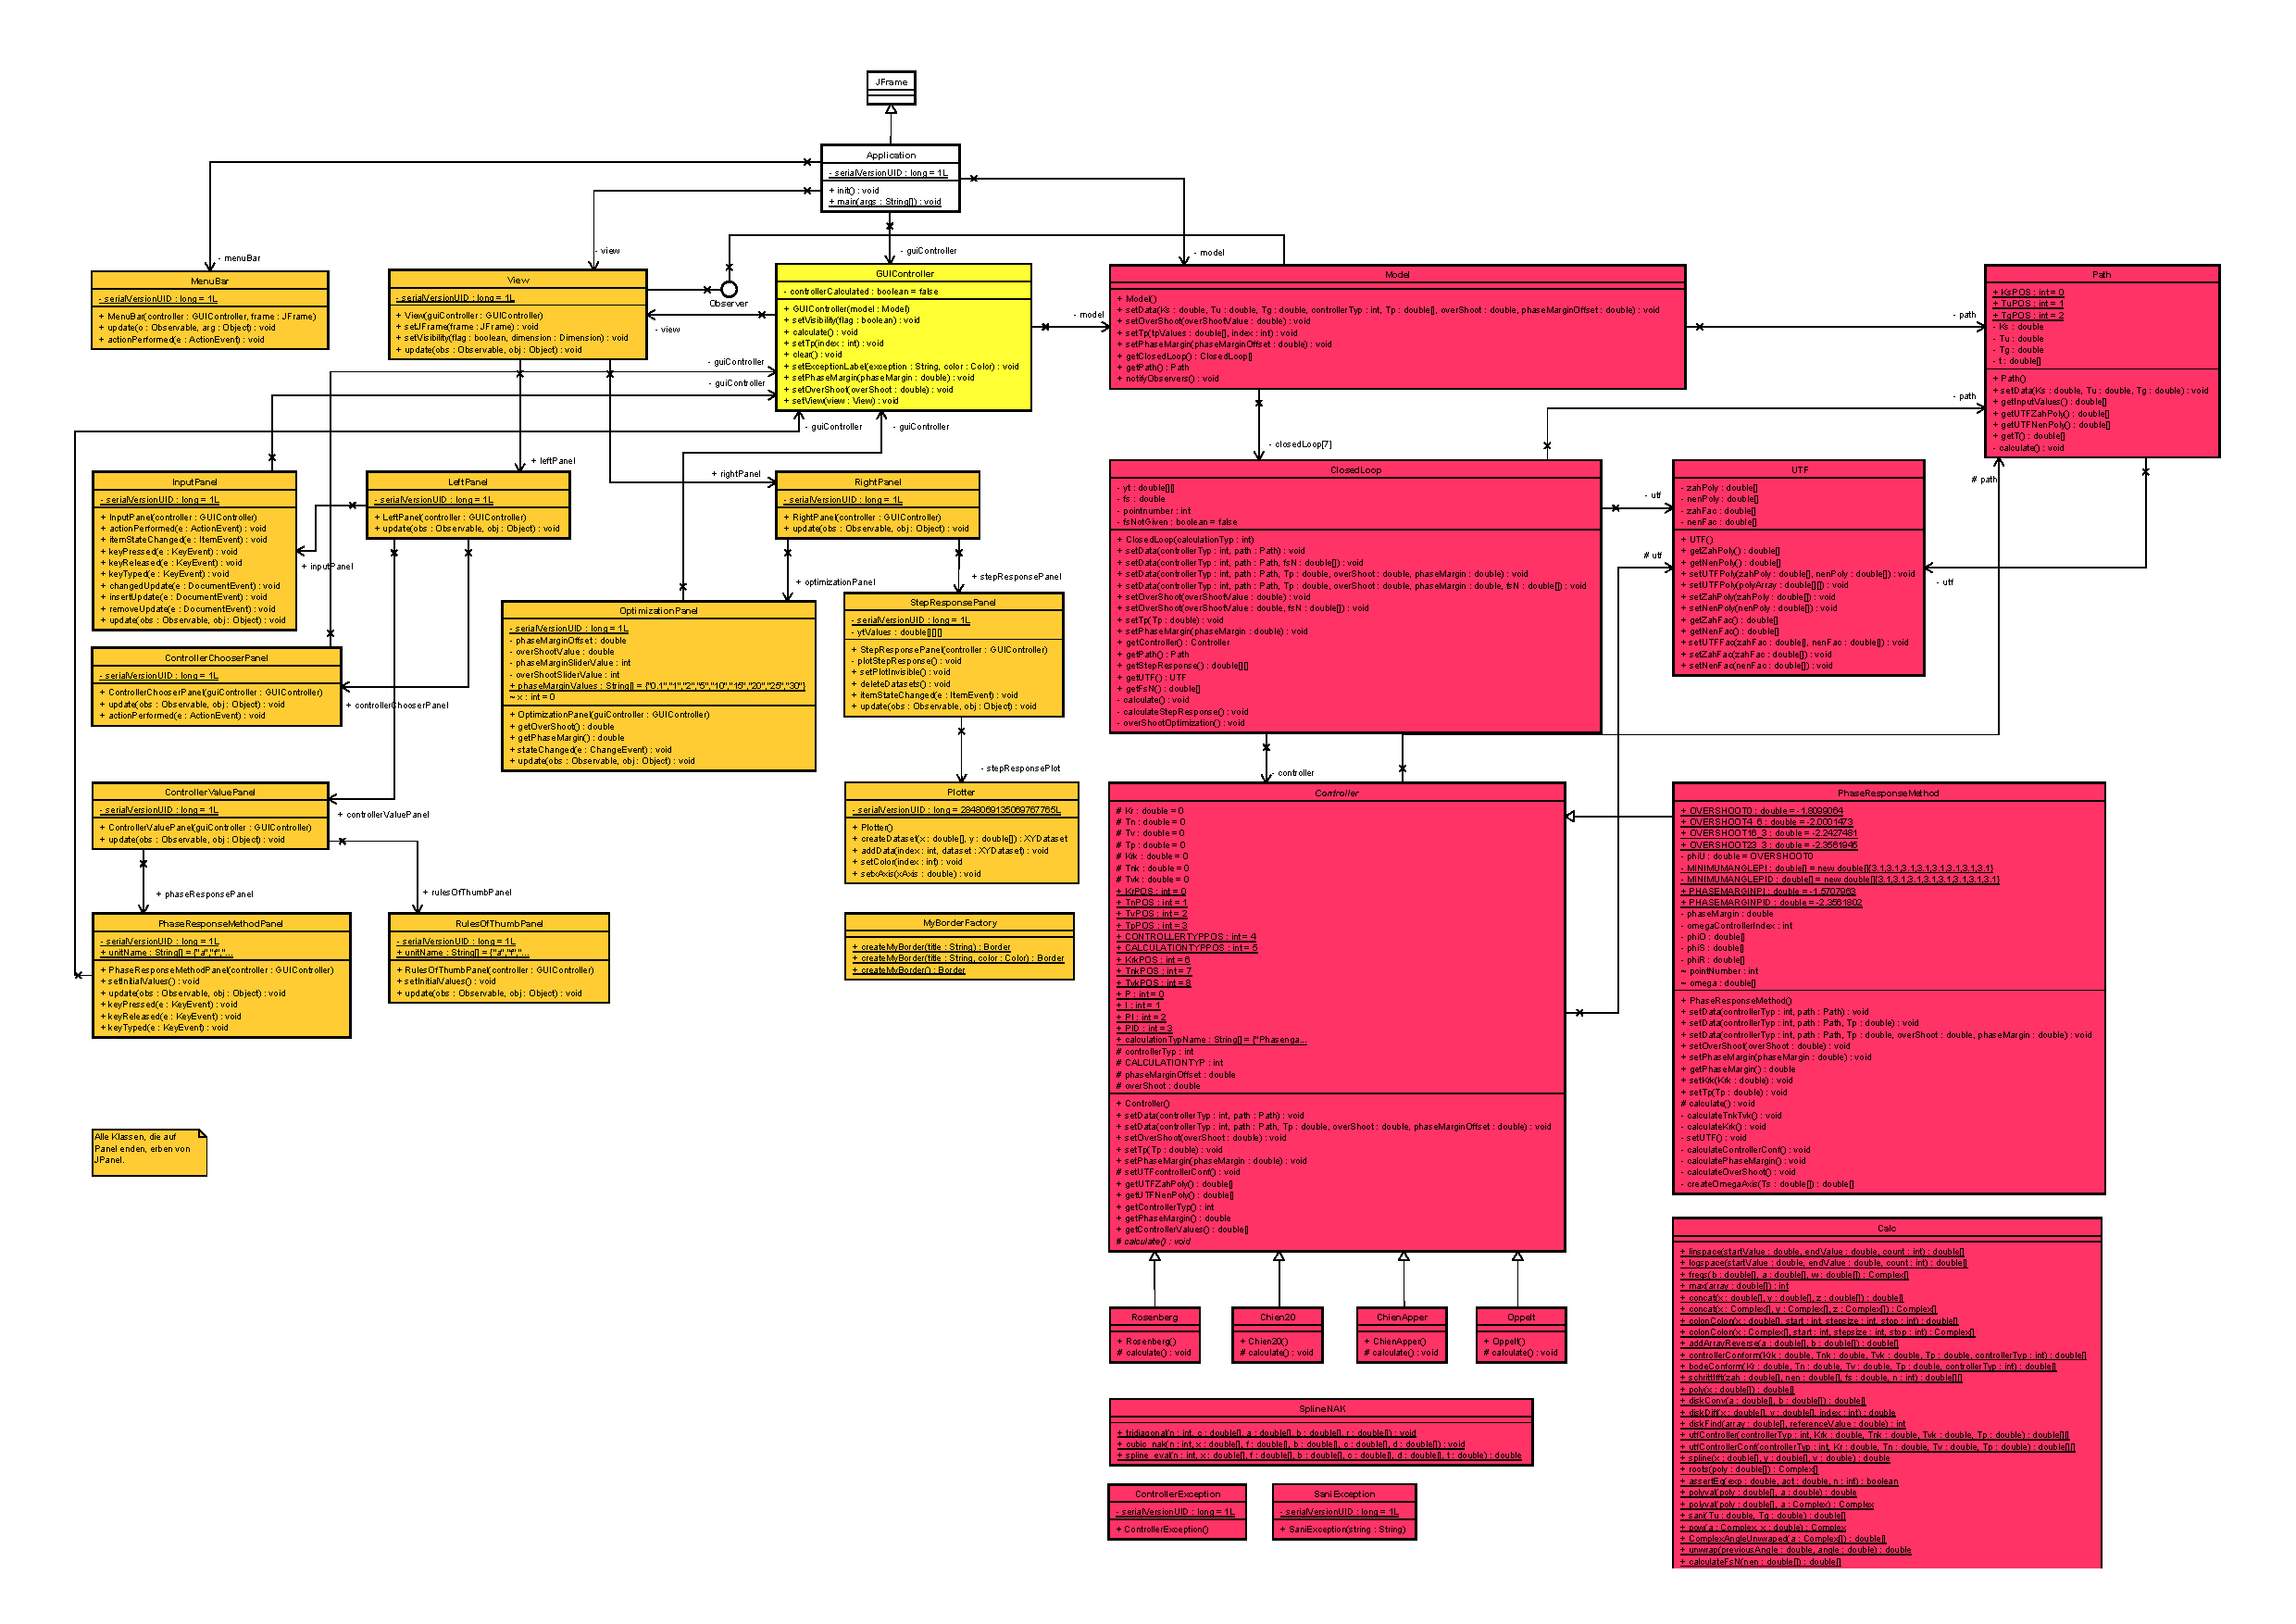
\includepdf[pages=1,scale=1]{images/klassendiagramm.pdf}

\setlength\paperheight{297mm}
\setlength\paperwidth{210mm}
\setlength\pdfpageheight{\paperheight}
\setlength\pdfpagewidth{\paperwidth}



% **************************************************************************** %
%\cleardoublepage
%\phantomsection
%\addcontentsline{toc}{section}{\listigurename}
%\listoffigures
% **************************************************************************** %

% **************************************************************************** %
\clearpage
\phantomsection
\addcontentsline{toc}{section}{\bibname}
\bibliography{bibliography/pflichtenheft_fachlicher_teil}{\bibliographystyle{bibliography/deIEEEtran.bst}}
% **************************************************************************** %

% **************************************************************************** %
\clearpage
\section*{Projektvereinbarung}
\label{sec:projektvereinbarung}
% **************************************************************************** %
\input{sections/projektvereinbarung.tex}


\end{document}
